\documentclass[runningheads,a4paper]{llncs}

\usepackage{amssymb}
\setcounter{tocdepth}{3}
\usepackage{graphicx}
\usepackage{url}
\usepackage{epsfig}


\urldef{\mailalex}\path|{alexander.toschev@gmail.com}|
\urldef{\mailmax}\path|{max.talanov@gmail.com}|

\begin{document}

\mainmatter

\title{Thinking Life Cycle as an implementation of machine understanding in IT maintenance domain}

\titlerunning{Thinking Lifecycle implementation in IT DID}

\author{Alexander Toschev\inst{1} \and Maxim Talanov\inst{2}}
\institute{Kazan State University, Chebotarev Research Institute of Mathematics and Mechanics\\
Universitetskaya 17, 420008 Kazan, Russia\\
\mailalex\\
\and
Kazan State University, Higher Institute for Information Technology\\
Universitetskaya 17, 420008 Kazan, Russia\\
\mailmax\\
}


\maketitle

\begin{abstract}
IT Infrastructure maintenance domain is a labor intensive process and contains many tools that help to solve a lot of every-day problems to support business operations. IT Infrastructure maintenance domain has a lot of primitive incidents that seems to be easy to automate. However there is still the gap to run business, operating support is provided by human specialists understanding and making decision how to implement even primitive incidents. One of the key factors in automation and in entire process is to understand input request consigned by human support specialist with cover functions this thinking processes:  correlation, simulation, reformulation. Using this model in 2006 Marvin Minsky has published his book "Emotion Machine" \cite{mmem} which was our inspiration and the base of implementation described below.

\keywords{AI, machine understanding, it outsourcing}

\end{abstract}

\section{Introduction}
We have been translated an ontology of the types of reflections that a system mind might make of itself. Our focus in particular on the negative—what are the ways that system criticizes its own activities.  We have implemented a ‘mental critics’ that we envision as populating the upper reflective levels of the system.

This implementation contains machine understanding model based on thinking model because human understanding is also based on human thinking. \\
In 2006 year Marvin Minsky has published his book “The Emotion Machine” where he describes model of human thinking dividing all actions into 3 categories:

\begin{enumerate}
 \item Critic
 \item Selector
 \item Way To Think
\end{enumerate}

\subsection{Critic}
Critic could be understood as probabilistic predicate. In real world when human faces the problem several critics are activated. In IT DID model\footnote{IT DID - IT Dynamic Infrastructure Domain - domain of IT services like remote Infrastructure support} there is Direct Instruction Critic (described below) that activates when direct instruction incident has been received. After activating critic returns Selector request.

Critic examples:

\begin{enumerate}
 \item Learned Reactive Critics.
 \item Deliberative Critics.
 \item Reflective Critics.
 \item Self-Reflective Critics.
 \item Self-Conscious Critics.
\end{enumerate}

\subsection{Selector}
Selector is capable of retrieving Resources (Critic or Way to think) from memory. Is the main component for memory(see below) processing.

\subsection{Way to think}
In our approach, a commonsense reasoning involves indirect mechanism for inferencing, but a vast of  specialized ways-to-think and suited for certain problem-types in IT Infrastructure domain problem solving strategies, such as:
\begin{enumerate}
 \item Knowing How — System doesn’t see most problems as problems at all, because it’s already know how to solve them (by calling to domain Knowledge Base).
 \item Analogy — Adapt a method have been used before (taken from work instructions, reports  and etc).
 \item Reformulation — When previous methods are fail, system tries to find a new way to describe the problem.
 \item Correlation — Matches inbound concepts with already known.
 \item Cry for Help — If none of  methods do not give a pass result, address for helping hand.
\end{enumerate}
Our architecture is designed to keep updating multiple representations of knowledge in parallel. This enables it to quickly switch between different ways-to-think. This means that the system will not get stuck because those alternate ways-to-think will be ready to take over when the present one runs into trouble. This is related to Minsky’s idea, where many views of an object are linked by their common parts to together form a more realistic or complete model than any individual view could form.

\emph{Practical example 1}, If incident is an automatically generated, system should process it using instruction book A.
\emph{Practical example 2}, If the problem symptoms already stored in the system knowledge base, use analogy to solve it.Way To Think in current implementation is a worker that modifies short term memory.

Worker components that actually changes the contents of short term memory(see below).

Way to think examples:
\begin{itemize}
 \item Simulation
 \item Correlation
 \item Reformulation
 \item Thinking by analogy
 \item …
\end{itemize}

\emph{Practical example 1}, “If incident is an automatically generated system should process it using instruction book A”.
\emph{Practical example 2}, “If the problem symptoms already stored in the system knowledge base, use analogy to solve it”.

\subsection{Thinking levels}

Minsky proposes six thinking level. Every thinking level has its own major functionality. Every next level is a more complex than previous.

\begin{enumerate}
 \item Instinctive
 \item Learned
 \item Deliberative
 \item Reflective
 \item Self-Reflective
 \item Self-Conscious
\end{enumerate}

First level contains inborn instincts and there are highest ideals and personal goals on the top level.

\subsection{Facts and statistics}
We have been inspired by the study of Incident Dump of Fujitsu GDC Russia Company\footnote{Russia, Kazan, Fujitsu GDC Russia, http://ru.fujitsu.com}. Study indicates that there are at lest 60\% of typical incidents that can be automated. Results of the analysis have been divided into 4 sub-domains:
\begin{enumerate}
 \item WINTEL (Microsoft Windows Operating System Management)
 \item Microsoft Active Directory Management.
 \item *NIX management (Linux, Unix operating systems).
 \item Storage Management.
\end{enumerate}

Every sub-domain has probability with which can be covered and \% of Tasks that can be covered. For example sub-domain WINTEL and task monitoring has 100\% covering with probability 1\footnote{Additional information and full report of results can be found on http://tu-project.com/for-business/}. On the other hand Operating tasks has covered with 96,875\% only. 

\section{Emotion machine prototype}
This implementation based on triple \emph{Critic-Selector-Way to think}. There are several critics, way-to-think and selector has been created:

\begin{enumerate}
 \item Natural language processing based on RelEx.
 \item Incident classification critics.
 \item Simulation.
 \item Reformulation.
 \item Correlation.
 \item Solution search.
\end{enumerate}

\subsection{Implemented thinking levels}

\begin{enumerate}
 \item Learned
 \item Deliberative
 \item Reflective
 \item Self Reflective
 \item Self Conscious
\end{enumerate}

Instinctive level is planned for future use as acceleration of automatically generated incidents.

\section{Thinking life cycle (TLC)}

The central idea behind our architecture is: using one method of solution, system can rapidly elevate to another. Thus, at the top level, our architecture is organized as follows. When the system encounters a problem, it first uses some knowledge about ‘problem-types’ to select some ‘way-to-think’ that might work.
The system TLC is capable of noticing problems in it's own activities. Our current architectural design also includes reflective levels beyond the deliberative level. Each reflective level(Reflective, Self Reflective, Self Concious) responding to problems in the levels beneath and includes:
\begin{itemize}
 \item Reflective — Reasoning about the recent deliberations of deliberative level, such as whether a subgoal has gotten the system closer to a supergoal or further away for processing.
 \item Self-Reflective — Reasoning about its activities with respect to large-scale thinking models of its abilities and limits, for example, what kinds of  IT domain objectives  the system knows, how it typically behaves in similar situations, and so forth.
 \item Self-Conscious — Reasoning about itself in relation to others entities. Emotional and feelings control.
\end{itemize}

TLC controls prototype thinking levels, short term memory, long term memory.

Typical workflow described in following steps:
\begin{itemize}
 \item Incident processing starts
 \item Suitable critic activates and returns selector request
 \item According to selector request Selector retrieves suitable Way to think
 \item Way To Think modifies data in Short term memory
 \item Process repeats until all the goals(see below) are satisfied
\end{itemize}

Thinking Lifecycle(TLC) run different resources simultaneously like a human specialists do. This way, different thinking levels are activated in parallel.

\subsection{Short Term Memory}
We present a general cognitive design based on reflective and deliberative level that uses distributed associative memories. The type of architecture we present is based on the interaction between an "attribute-object selector" and an "critic filter” of successive evoked objects, with the intermediation of a working (short-term) memory.
Ways to think actively operates with common data that are stored in short term memory or a context. Short term memory contains a set of current processing data required for every component of the Selector -> Critic -> Way to think triple: domain model, last processing result e.t.c.

\subsection{Long Term Memory}
In contrast of Short Term Memories, Long Term Memories are viewed as I/O units responsible for translating data of short term memory processed result and reflected into previously remembered states, and vice-versa. After several thinking cycles data from short term memory is merged with data in long term memory.

\subsection{Domain model}
Domain model is a set of current knowledge for specific scope: known problems, solutions, existing concepts, existing how-tos, critics, way to think.\\

\section{Thinking Model}
The picture below shows Thinking process example

\begin{figure}

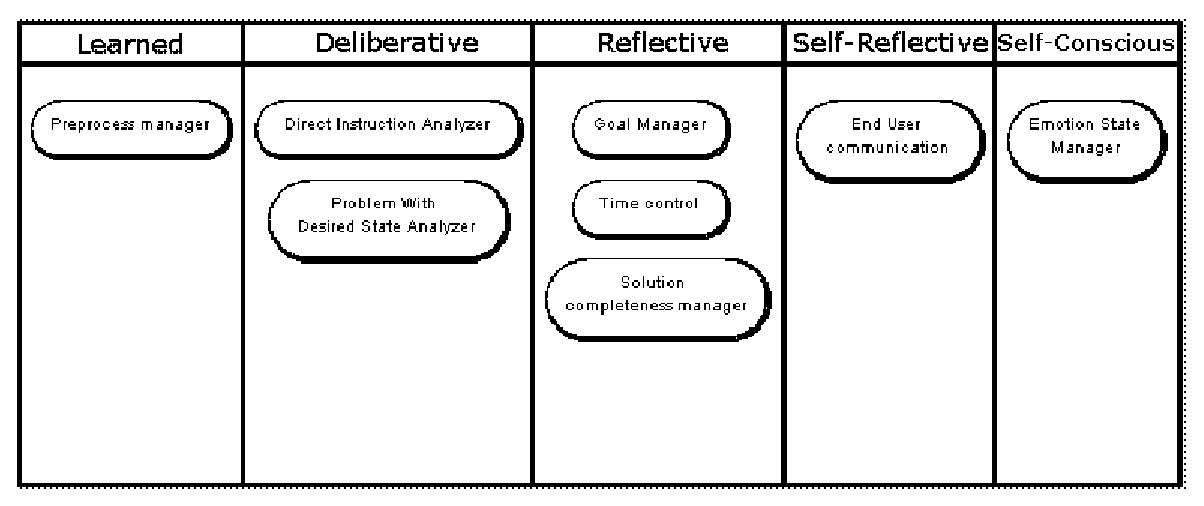
\epsfig{file=tuactivity5.eps, height=150px, width=340px}

\caption{Thinking process example}
\end{figure}
In our view human-level learning requires a not standard architectural approach that is tightly connected to the rest of thinking. Beside resolution problem as a functional goal of the system it also is focused on the ‘credit assignment problem’ — system could decide how to improve itself, especially as problems for resolution gets more complicated.  As the system grows, that requires a more and more elaborate self-model implementation, so that the reflective layers of the system can try to predict the effects of changes it might make to itself. Powerful learning is enabled by a powerful ability to reflect.


\subsection{Learned}

\subsubsection{Process manager.} This manager activates several Way To Think to perform initial incident processing. The goal of this critic is to produce semantic network of the incident. There are several Way To Think:
\begin{itemize}
 \item Auto Correction of spelling
 \item Synonymic search
 \item Annotation – finding existing concepts in Knowledge Base
\end{itemize}

\subsection{Deliberative}

Incident processing on the deliberative level main activities: select suitable analyzers from memory for learned level and search proper solutions.

\subsubsection{Direct Instruction Analyzer.} This Critic activates when direct instruction detected in incoming request. For example, “Please install MS Office 2012” is a direct instruction for system.
\subsubsection{Problem With Desired State Analyzer.} Critic activates when problem with desired state detected by the system. For example, “I have Internet Explorer 8 installed, but finance department requested Internet Explorer 7”.

\subsection{Reflective}

System sets processing goals, performs time control, runs solution completeness manager.

\subsubsection{Goal manager.} Processing goals mechanism is used to increase performance of incident processing. Goals are links between critics and way to think. Main goal is to Help User. Other goals, that derived from it, for example:
\begin{itemize}
 \item Resolve incident
 \item Understand incident type
 \item Model Direct Instruction
\end{itemize}
Goal manager links way to think with actions(critics or way to think) and finds required for current goal processing way to think.

\subsubsection{Time control.} Time control tracks time of a incident processing. (SLA\footnote{SLA-Service Layer Agreement, the period of time while incident should be processed} in terms of IS domain)

\subsubsection{Solution completeness manager.} This manager runs solution analysis to check if solution found is complete.

\subsection{Self-reflective}
System controls actions of lower levels like: initialize short term memory or start time control. All communication with user is also managed on this level, for example by Do Not Understand Manager.\\
Practical example: System doesn't know concept "Opera software". Using the clarification request system learns new concept.

\subsubsection{Dialog mode.}
Important part of prototype implementation is an ability to work in Dialog mode with end user. When system faces with problem (e.g. unknown concept) it solves this issue asking help from human specialist.

\subsection{Self-conscious}
This level is a top in hierarchy. On this level system tracks and sets the Emotional State. For example reacting for long incident processing system changes emotional state to anxious to allocate more resources for processing.

\subsection{Training}
System trains during operation via communication with human specialist. However, current prototype also works in separate training mode. System perceives all input data as training requests in it. On the initial stage system filled with base concepts:
\begin{itemize}
 \item Concept
 \item Action
 \item Form of politeness
\end{itemize}

For example, let's take "Please install Firefox Incident". One of the possible learning curve for this incident is: "Firefox is a browser. Install is an action. Please is a form of politeness." After learning it system cans process incident\footnote{Additional information available here http://tu-project.com/student-book/}. Current version of project is 1.1 "Nemesis"\footnote{Full roadmap here http://tu-project.com/roadmap/}

\section{Initial processing results}

According to initial processing results approx. 61\% of incidents can be understood. 

\section{Conclusions}

The main goal of described prototype is feasibility study of application of "Emotion Machine" \cite{mmem} in IT Maintenance Domain in boundaries of the cycle from processing incident in natural language(English) up to machine understood request. In future: found and applied solution. Prototype is capable of evolving during the operation via training option.

\begin{thebibliography}{4}

\bibitem{lili}
Liu H., Lieberman H.:
Metafor: Visualizing Stories as Code.
Cambridge, MIT Media Laboratory  (2005).

\bibitem{runo}
Russel S., Norvig P.:
Artificial Intelligence. A Modern approach.
Pearson (2010).

\bibitem{mmem}
Minsky M.:
The Emotion Machine.
Simon \& Schuster Paperbacks  (2006).

\end{thebibliography}

\end{document}

